\documentclass[conference]{acmsiggraph}

\usepackage{cleveref}

\title{The Title of Your Paper Goes Here}

%%%%%%%%%%%%%%%%%%%%%%%%%%%%
% authors
%%%%%%%%%%%%%%%%%%%%%%%%%%%%
\author{
	Felix Manke\thanks{e-mail: felix.manke@campus.lmu.de}\\LMU Munich
	\and
	Tibor Goldschwendt\thanks{e-mail: goldschwendt@cip.ifi.lmu.de}\\LMU Munich
	\and
	Oleg Maltsev\thanks{e-mail: ga49bof@mytum.de}\\TU Munich
}
	
\pdfauthor{Felix Manke, Tibor Goldschwendt}

\keywords{radiosity, global illumination, constant time}

\begin{document}

%% \teaser{
%%   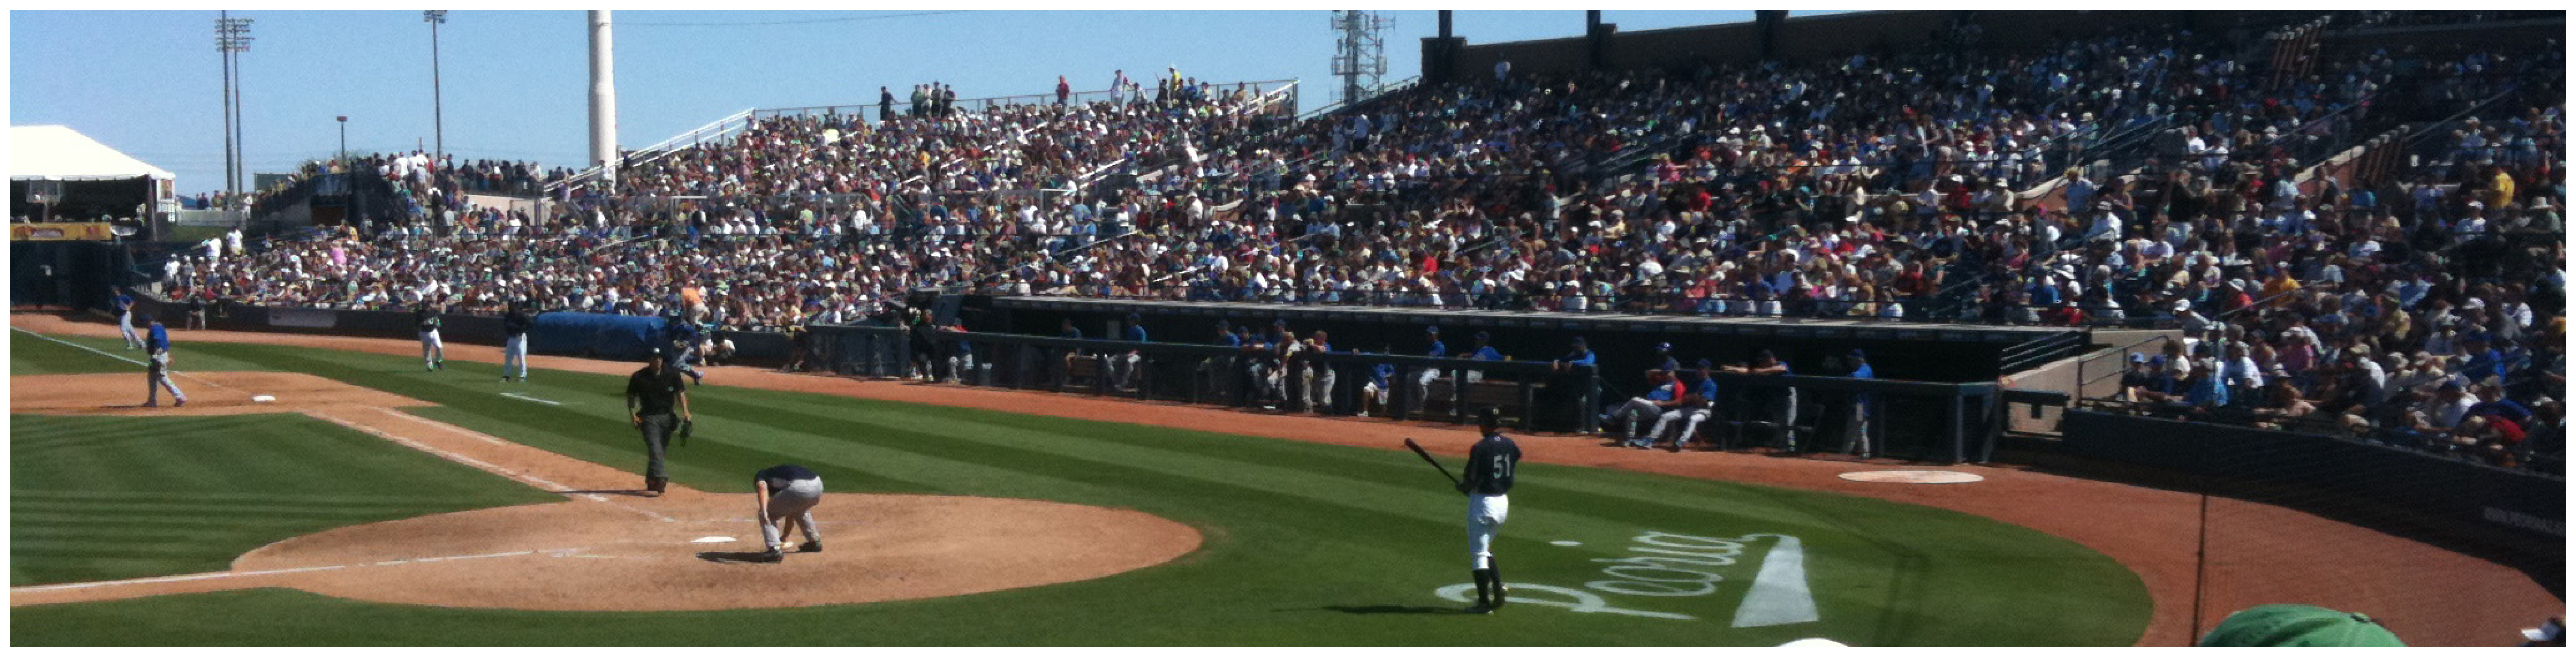
\includegraphics[height=1.5in]{images/sampleteaser}
%%   \caption{Spring Training 2009, Peoria, AZ.}
%% }

\maketitle


%%%%%%%%%%%%
% ABSTRACT %
%%%%%%%%%%%%

\begin{abstract}

\end{abstract}

\copyrightspace




%%%%%%%%%%%%%%%%
% INTRODUCTION %
%%%%%%%%%%%%%%%%

\section{Introduction}

\begin{itemize}
\item motivation
\item{
	general description of the project
	\begin{itemize}
	\item what is it\\
	 ($\rightarrow$ introductory text from wiki... separation of senses, visual, tactile, ...)
	\item dark room side (explanation of dark room: what happens there, what does the user do. Not too technical\\
	 $\Rightarrow$ only the concept)
	\item communication
	(point out, that data gets transmitted over to the cave so that there is a spatial separation as well)
	\item CAVE-side\\
	(how does the interaction in the cave look like? what happens there? How does the room-user affect the cave-environment and vice versa...)
	\end{itemize}
}
\item entire team\\
	  (describe, who worked on the project... what about a complete list of all names in the appendix maybe, like credits in a movie or video game?)
\item aspects: arts vs. technology\\
		(combination of both worlds, merging the best aspects, creating an immersive installation)
\item how we find the concept\\
		(description of the development process $\Rightarrow$ time (October till March... still ongoing to prepare it for future exhibitions...), presence meetings in Munich and Linz aka. Workshops, several Skype-Meetings, different approaches and ideas (interactive table, visualising time, ... , finally: separation of senses) 
\item purpose of this paper
\end{itemize}

\section{Implementation}




%%%%%%%%%%%%%%%%%%%%%%%%%%%%
% APPLICATION ARCHITECTURE %
%%%%%%%%%%%%%%%%%%%%%%%%%%%%

\subsection{General Application Architecture}
\textit{Graphic / diagram} to visualize the overall system architecture (room-components, network, cave-components)
\begin{itemize}
\item brief description of components
\end{itemize}




%%%%%%%%%%%
% NETWORK %
%%%%%%%%%%%

\subsection{Network}
\begin{itemize}
\item introduction
\item{
	used technologies
	\begin{itemize}
	\item Liblo + OSC
	\end{itemize}
}
\item evolution over time
\item{
	detailed description
	\begin{itemize}
	\item UML
	\item programming language, libraries...
	\item API
	\item implementation, code examples, algorithms,...
	\end{itemize}
}
\end{itemize}





%%%%%%%%%%%%%%%%%
% VISUALISATION %
%%%%%%%%%%%%%%%%%

\subsection{Visualisation}
\begin{itemize}
\item introduction
\item{used technologies
	\begin{itemize}
	\item{CAVE
		\begin{itemize}
		\item some technical details on the cave
		\item ideally some pictures/figures...
		\end{itemize}
	}
	\item{OpenSG
		\begin{itemize}
		\item{ What is OpenSG?
			\begin{itemize}
			\item rough description
			\item why do we use it?
			\item some references (OpenSG, docu, etc ...)
			\end{itemize}
		}
		\item{The Scenegraph
			\begin{itemize}
			\item figure / diagram
			\item description of all nodes
			\item reasons for this layout of the scenegraph
			\end{itemize}
		}
		\end{itemize}
	}
	\item{GLUT
		\begin{itemize}
		\item{What is the OpenGL Utility Toolkit?
			\begin{itemize}
			\item rough description
			\item some references
			\end{itemize}
		}
		\item{What is it used for?
			\begin{itemize}
			\item basic GLUT window to create program/update loop
			\item receive mouse and keyboard input
			\item ...?
			\end{itemize}
		}
		\item How is it implemented?
		\end{itemize}
	}
	\item{CaveSceneManager
		\begin{itemize}
		\item What is the CaveSceneManager?
		\item some references
		\item why do we use it / what do we need it for?
		\item how did we implement it?
		\end{itemize}
	}
	\item don't forget to mention the 3D-models coming from the artists, build in 3D-Max and Maya, I guess...
	\end{itemize}
}
\item{The Avatar
	\begin{itemize}
	\item{Introduction
		\begin{itemize}
		\item{What is an Avatar?
			\begin{itemize}
			\item some background information on the concept of avatars
			\item including some references
			\end{itemize}
		}
		\item{Why do we need it / What do we use it for?
			\begin{itemize}
			\item visualizing the remote user and his movement through space
			\item allowing for interaction with the remote user via this virtual representaion
			\end{itemize}
		}
		\end{itemize}			
	}
	\item{Design of the Avatar
		\begin{itemize}
		\item what functionality was needed
		\item how should the avatar behave
		\item{what should it look like?
			\begin{itemize}
			\item human-like representation
			\item but still abstract, artificial
			\end{itemize}
		}
		\item{what should the interaction with the avatar look like?
			\begin{itemize}
			\item approaching, touching, hitting,...
			\item interaction through movement in space
			\end{itemize}
		}
		\item{what implications came from this for the implementation of the avatar?
			\begin{itemize}
			\item needed to look human-like
			\item needed to be able to react visually to interaction
			\item on the one hand "large scale proximity" $\Rightarrow$ the user moving towards/away from the avatar
			\item on the other hand "small scale proximity" $\Rightarrow$ the user touching different parts of the avatar
			\end{itemize}
		}
		\end{itemize}			
	}
	\item{Implementation
		\begin{itemize}
		\item UML
		\item{visuals
			\begin{itemize}
			\item human shape / silhouette
			\item rotating cubes / orbits
			\item exchange of cubes with the ground
			\item vest
			\item varying size depending on distance between user and avatar
			\end{itemize}
		}
		\item{interaction
			\begin{itemize}
			\item interaction by proximity
			\item changing size (far away $\Rightarrow$ diffuse large cube cloud; close $\Rightarrow$ defined human shape, plus: vest becomes visible)
			\item pulsating cubes(touch, hit, bump)
			\end{itemize}
		}
		\item components/variables/methods
		\item description of all subclasses
		\item usage / API
		\item{network
			\item what gets send over the network?
			\item what gets received?
			\item ... where to put this in the doc? maybe here just a reference to the network chapter?
		}
		\end{itemize}		
	}
	\end{itemize}
}
\item{The Virtual World
	\begin{itemize}
	\item visuals
		\begin{itemize}
		\item some details on size, purpose, etc. ...
		\item screenshots
		\end{itemize}
	\item creation process
		\begin{itemize}
		\item built in 3DMax / Maya / Blender
		\item import into OpenSG $\Rightarrow$ plus code snippet
		\end{itemize}
	\item movement /navigation
		\begin{itemize}
		\item Wand to lead direction
		\item Joystick to move around
		\item tracking of wand to move the user's hand around for interaction (touching, hitting,...)
		\end{itemize}
	\item movement constraints
		\begin{itemize}
		\item maximum speed
		\item borders for navigation
		\end{itemize}
	\end{itemize}
}
\item (evolution over time ?)
\item{
	detailed description
	\begin{itemize}
	\item UML, Code
	\item programming language, libraries...
	\item API
	\item implementation, code examples, algorithms,...
	\end{itemize}
}
\end{itemize}





%%%%%%%%%%%%%%%
% INTERACTION %
%%%%%%%%%%%%%%%

\subsection{Interaction}
\begin{itemize}
\item introduction
\item{ used technologies
	\begin{itemize}
	\item{IR tracking system
		\begin{itemize}
		\item{description of the technical Cave-Setup for Headtracking
			\begin{itemize}
			\item infrared lights
			\item cameras
			\item figure / blueprint of tracking setup in cave
			\item markers on 3D-glasses (picture of 3D-shutterglasses with markers on it)
			\item markers on Wand
			\end{itemize}
		}
		\item{what can be achieved by this?
			\begin{itemize}
				\item Headtracking $\Rightarrow$ correct perspective
				\item Tracking of Wand position $\Rightarrow$ position of user's hand
				\item immersion
				\item interaction
				\item ...?
			\end{itemize}		
		}
		\end{itemize}
	}
	\item{Wand
		\begin{itemize}
		\item short description of the Wand and its features
		\item figure / picture of the Wand
		\item references (manufacturer / documentation)
		\end{itemize}
	}
	\item{VRPN
		\begin{itemize}
		\item short description of the framework/library
		\item references
		\item what do we use it for?
		\item how is it implemented?
		\end{itemize}
	}
	\end{itemize}
}
\item evolution over time
\item{
	detailed description
	\begin{itemize}
	\item UML
	\item programming language, libraries...
	\item API
	\item implementation, code examples, algorithms,...
	\end{itemize}
}
\end{itemize}

\section{Conclusion \& Further Extensions}



%%%%%%%%%%%%%%%%%%%%%%%
% FORMATTING EXAMPLES %
%%%%%%%%%%%%%%%%%%%%%%%


\textit{\textbf{Formatting examples (will be deleted later on...)}}

\cref{SEC:CFE}\\
\Cref{SEC:CFE}

(\textit{see \cref{FIG:SAMPLE}})

\label{SEC:CFE}

\begin{equation}
 \sum_{j=1}^{z} j = \frac{z(z+1)}{2}
\end{equation}

\begin{eqnarray}
x & \ll & y_{1} + \cdots + y_{n} \\
  & \leq & z
\end{eqnarray}

\begin{figure}[ht]
  \centering
  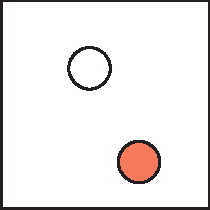
\includegraphics[width=1.5in]{images/samplefigure}
  \caption{Sample illustration.}
  \label{FIG:SAMPLE}
\end{figure}

\section*{Acknowledgements}

To my mum, my dad, and the dog. 

\bibliographystyle{acmsiggraph}
\bibliography{template}
\end{document}
